\documentclass{article}

\usepackage{tikz}
\usepackage{pgfplots}
\usetikzlibrary{calc,3d,decorations.markings, backgrounds, positioning,intersections,shapes}

\begin{document}
\thispagestyle{empty}
\begin{figure}[H]
\centering
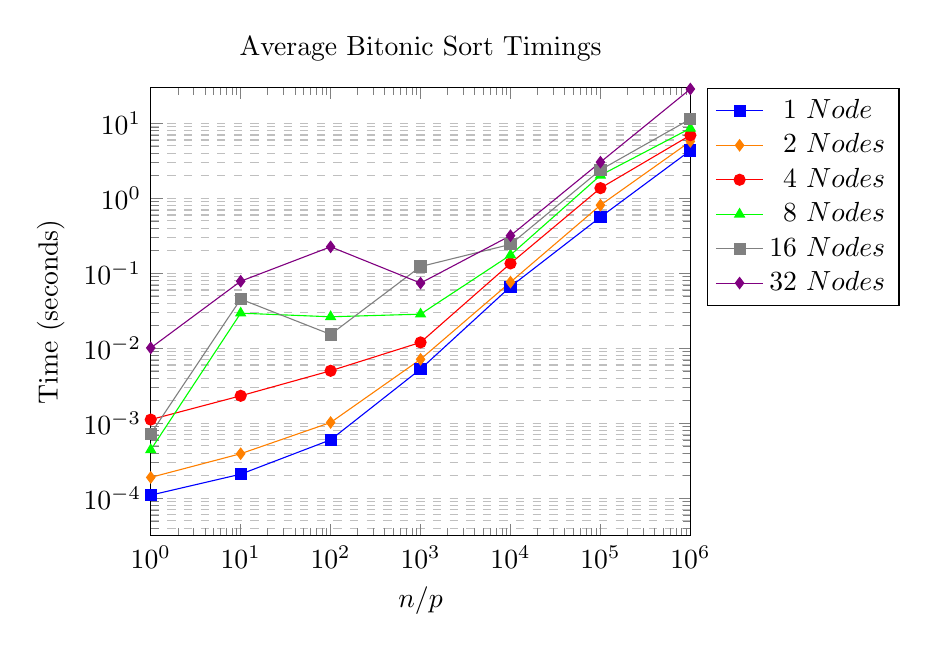
\begin{tikzpicture}
\begin{axis}[
    title={Average Bitonic Sort Timings}, xlabel={$n/p$}, ylabel={Time (seconds)}, xmin=1, xmax=1000000, ymin=0, ymax=30, xmode=log, ymode=log,legend pos=outer north east,ymajorgrids=true,yminorgrids=true,grid style=dashed,]%ytick={0, .1, .2, .3, .4, .5, .6, .7, .8, .9, 1.0},]
\addplot[color=blue, mark=square*,]
        coordinates{(1,.000110197)(10,.000209665)(100,.000602054)(1000,.005284738)(10000,.06643854)(100000,.5624708)(1000000,4.348568)};
\addplot[color=orange, mark=diamond*,]
        coordinates{(1,.00018996)(10,.000393212)(100,.001024666)(1000,.007139028)(10000,.0763502)(100000,.810724)(1000000,5.7469225)};
\addplot[color=red, mark=*,]
        coordinates{(1,.00112033)(10,.0023266592)(100,.005016398)(1000,.0119927)(10000,.13549075)(100000,1.36762)(1000000,6.9464775)};
\addplot[color=green, mark=triangle*,]
        coordinates{(1,.000442743)(10,.029427207)(100,.026337)(1000,.028541933)(10000,.175502333)(100000,2.028616667)(1000000,8.586426667)};
\addplot[color=gray, mark=square*,]
        coordinates{(1,.000725031)(10,.04526545)(100,.015321033)(1000,.123152933)(10000,.243317)(100000,2.397353333)(1000000,11.40923333)};
\addplot[color=violet, mark=diamond*,]
        coordinates{(1,.010123428)(10,.07847924)(100,.225703)(1000,.07412014)(10000,.31788654)(100000,3.038054)(1000000,28.71392)};
\legend{$\phantom{1}1\ Node\phantom{s}$, $\phantom{1}2\ Nodes$, $\phantom{1}4\ Nodes$, $\phantom{1}8\ Nodes$, $16\ Nodes$, $32\ Nodes$}
\end{axis}
\end{tikzpicture}
\caption{Each node had 16 MPI processes.}
\label{fig:timings}
\end{figure}
\end{document}